\section{Appendix}
\appendix

\section{System Overview}
\label{sec:SystemOverview}
\begin{figure}[H]
\centering
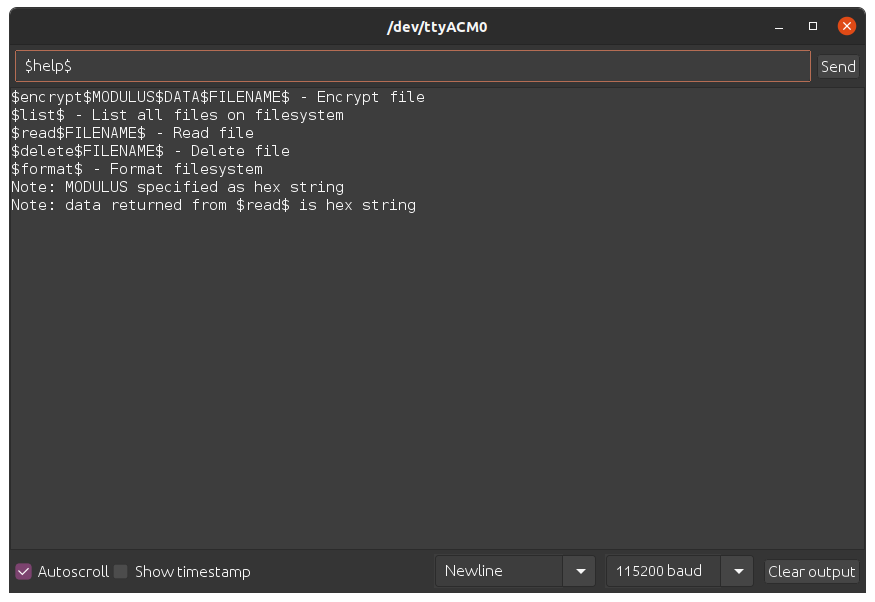
\includegraphics[width=1\columnwidth]{Figures/Fig_80.png}
\caption{Result of \$help\$ command in Arduino serial monitor.}
\label{fig:gantt}
\end{figure}

A link to a video demonstration of the system can be found \href{https://www.youtube.com/watch?v=u4TFHCfZJ7M}{here}. 

\section{Firmware}
\subsection{Auxiliary MCU}
\subsubsection{File System - fs.h}
\label{sec:fsh}
\href{https://github.com/spacehen/EEE4022F/blob/main/Firmware/Auxiliary\%20MCU/fs.h}{fs.h} is the C++ header file for the filesystem and contains public API definitions. 
\subsubsection{File System - fs.cpp}
\label{sec:fscpp}
\href{https://github.com/spacehen/EEE4022F/blob/main/Firmware/Auxiliary\%20MCU/fs.cpp}{fs.cpp} is the main C++ source file containing the filesystem implementation.
\subsubsection{Crypto Module - rsa.h}
\label{sec:rsah}
\href{https://github.com/spacehen/EEE4022F/blob/main/Firmware/Auxiliary\%20MCU/rsa.h}{rsa.h} is the C++ header file containing public cryptographic function definitions (Crypto Module).
\subsubsection{Crypto Module - rsa.cpp}
\label{sec:rsacpp}
\href{https://github.com/spacehen/EEE4022F/blob/main/Firmware/Auxiliary\%20MCU/rsa.cpp}{rsa.cpp} is the C++ source of the RSA-1024 implementation (Crypto Module).
\subsubsection{Communication Logic - main.ino}
\label{sec:comm}
\href{https://github.com/spacehen/EEE4022F/blob/main/Firmware/Auxiliary\%20MCU/main.ino}{main.ino} is the C++ source for the communication logic and main entry point of the auxiliary MCU.
\subsection{USB Driver MCU}
\label{sec:usbmcu}
\subsubsection{Serial Driver - serial.h}
\href{https://github.com/spacehen/EEE4022F/blob/main/Firmware/USB\%20Driver\%20MCU/USB/serial.h}{serial.h} is the C header for the serial portion of the USB driver.
\subsubsection{Serial Driver - serial.c}
\href{https://github.com/spacehen/EEE4022F/blob/main/Firmware/USB\%20Driver\%20MCU/USB/serial.c}{serial.c} is the C source file for the serial portion of the USB driver.
\subsubsection{USB Config - usbconfig.h}
\href{https://github.com/spacehen/EEE4022F/blob/main/Firmware/USB\%20Driver\%20MCU/USB/usbconfig.h}{usbconfig.c} is the C header to configure the V-USB driver.
\subsubsection{USB Driver - main.c}
\href{https://github.com/spacehen/EEE4022F/blob/main/Firmware/USB\%20Driver\%20MCU/USB/main.c}{main.c} is the entry point for the USB driver MCU.


\section{Software}
\subsection{Native host}
\subsubsection{Main Entry - main.c}
\label{sec:mainc}
\href{https://github.com/spacehen/EEE4022F/blob/main/Software/Nativehost/main.c}{main.c} is the main C++ source file for the native host client. 
\subsection{Browser Extension}
\label{sec:browser11}
\subsubsection{Background Script - background.js}
\label{sec:back}
\href{https://github.com/spacehen/EEE4022F/blob/main/Software/Browser\%20Extension/background.js}{background.js} is the background script of the browser extension that manages communication between the native host as well as passing messages to the UI popup.
\subsubsection{UI Script - script.js}
\href{https://github.com/spacehen/EEE4022F/blob/main/Software/Browser\%20Extension/script.js}{script.js} is the main script of the extension UI popup.
\subsubsection{UI - ui.html}
\href{https://github.com/spacehen/EEE4022F/blob/main/Software/Browser\%20Extension/ui.html}{ui.html} is the HTML definition of the UI popup.
\subsubsection{Extension Manifest - manifest.json}
\href{https://github.com/spacehen/EEE4022F/blob/main/Software/Browser\%20Extension/manifest.json}{manifest.json} is permissions file for the UI popup.

\section{Schematics}
\subsection{USB Driver MCU}
\label{sec:appd1}
\begin{figure}[H]
\centering
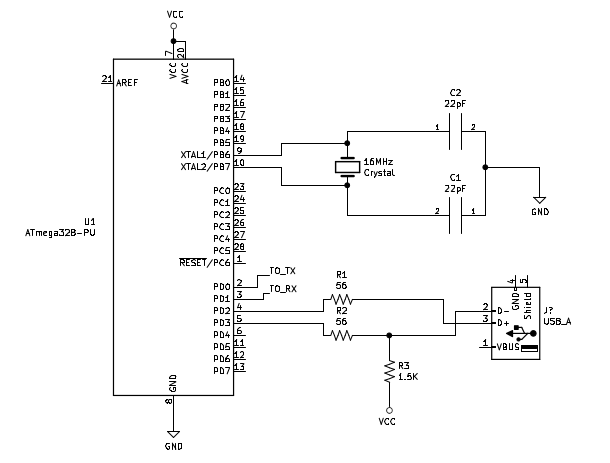
\includegraphics[width=0.9\columnwidth]{Figures/Fig_23.png}
\caption{USB driver schematic. V(cc) connected to ISP 3.3V.}
\label{fig:gantt}
\end{figure}
\subsection{Auxiliary MCU}
\label{sec:appd2}
\begin{figure}[H]
\centering
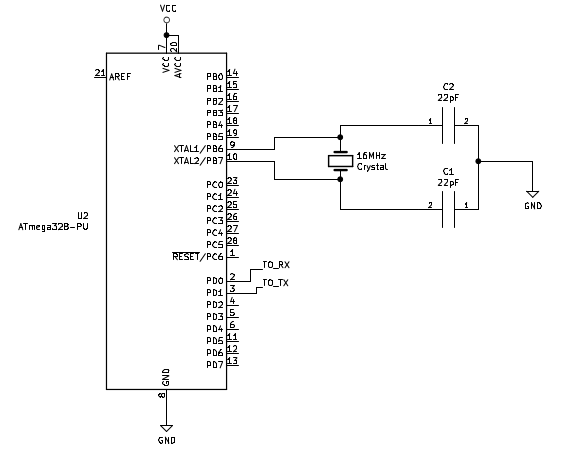
\includegraphics[width=0.9\columnwidth]{Figures/Fig_25.png}
\caption{Auxiliary MCU schematic. V(cc) connected to ISP 3.3V.}
\label{fig:gantt}
\end{figure}

\section{Experiments}
\subsection{Experiment 1}
\label{sec:exp1}
\lstinputlisting{Source/exp1.py}
\subsection{Experiment 2}
\label{sec:exp2}
\lstinputlisting{Source/exp2.c}
\subsection{Experiment 3}
\label{sec:exp3}
\lstinputlisting{Source/exp3.c}
\subsection{Python Timer}
\label{sec:timerp}
\lstinputlisting{Source/timer.py}
\subsection{C Timer}
\label{sec:timerc}
\lstinputlisting{Source/timer.c}
\section{Store Credential Flow}
\label{sec:credflow}
\begin{figure}[H]
\centering
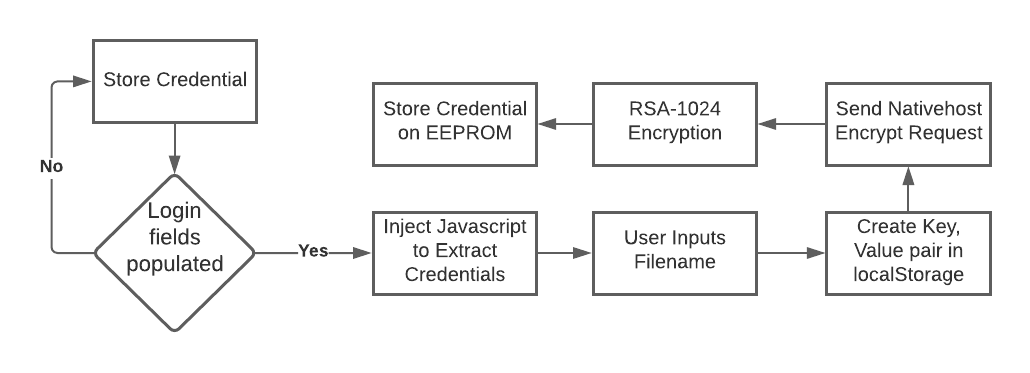
\includegraphics[width=0.9\columnwidth]{Figures/Fig_55.png}
\caption{'Store Credential' control flow.}
\label{fig:gantt}
\end{figure}

\section{USB Driver Flow}
\label{sec:usbflow}
\begin{figure}[H]
\centering
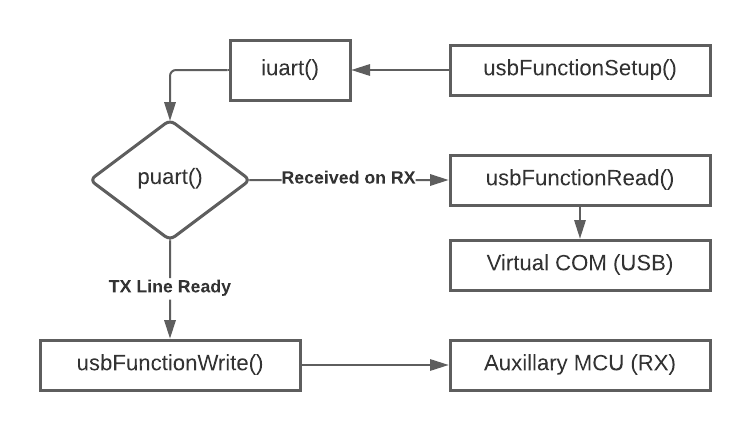
\includegraphics[width=0.7\columnwidth]{Figures/Fig_61.png}
\caption{USB driver control flow. With respect to the driver MCU.}
\label{fig:gantt}
\end{figure}

\section{Encryption/Decryption Flow}
\label{sec:eflow}
\begin{figure}[H]
\centering
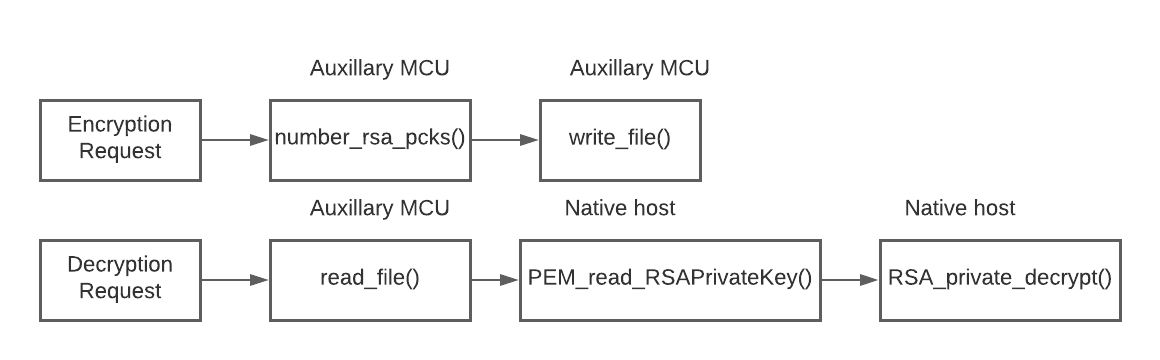
\includegraphics[width=1\columnwidth]{Figures/Fig_81.png}
\caption{Encryption/Decryption control flow.}
\label{fig:gantt}
\end{figure}

\section{Browser Extension}
\label{sec:bext1}
\begin{figure}[H]
\centering
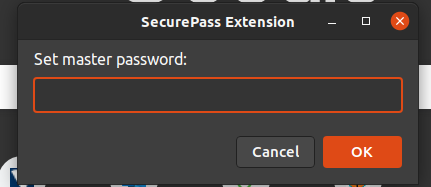
\includegraphics[width=0.6\columnwidth]{Figures/Fig_82.png}
\caption{Browser master authentication window.}
\end{figure}

\label{sec:bext2}
\begin{figure}[H]
\centering
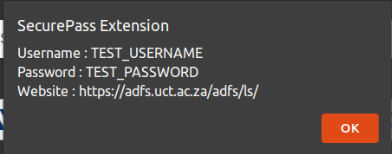
\includegraphics[width=0.55\columnwidth]{Figures/Fig_84.png}
\caption{Result when decrypt icon is selected.}
\end{figure}


